\documentclass[border=6pt]{standalone}
% Shared preamble for web figures.  Each figure is a standalone .tex that
% \input's this file; scripts/make-figures.sh turns it into an SVG.
% Handouts pull the same file with \fig{Unit_X/<name>}.
\usepackage[T1]{fontenc}
\usepackage{helvet}
\renewcommand{\familydefault}{\sfdefault}
\renewcommand{\ttdefault}{pcr}  % Courier: a real Type 1 typewriter font
\usepackage{amsmath}
\usepackage{tikz}
\usetikzlibrary{arrows.meta,positioning,calc,shapes.symbols,shapes.geometric}

% Who makes the rules is the point of most diagrams in this book, so the
% colors mean the same thing everywhere: blue is a person, orange is the
% computer, green is an answer, pink is the human brain.
\definecolor{person}{HTML}{2C6FAE}
\definecolor{machine}{HTML}{D35400}
\definecolor{result}{HTML}{1E8449}
\definecolor{brainpink}{HTML}{C2185B}
\definecolor{ink}{HTML}{2C3E50}

\tikzset{
  doodle/.style={line width=1.5pt, line cap=round, line join=round, draw=ink},
  box/.style={draw, rounded corners=5pt, line width=1.1pt, align=center,
              inner sep=7pt, minimum height=1.0cm, font=\small},
  personbox/.style={box, draw=person, fill=person!10},
  machinebox/.style={box, draw=machine, fill=machine!10},
  resultbox/.style={box, draw=result, fill=result!10},
  plainbox/.style={box, draw=ink!70, fill=ink!4},
  flow/.style={-{Stealth[length=8pt]}, line width=1.4pt, draw=ink},
}

% A person (blue) and a robot head (orange) as small icons.
% \personicon{x}{y}{scale}   \roboticon{x}{y}{scale}
\newcommand{\personicon}[3]{%
  \begin{scope}[shift={(#1,#2)}, scale=#3]
    \fill[person] (0,0.62) circle (0.28);
    \fill[person, rounded corners=6pt] (-0.42,-0.55) rectangle (0.42,0.28);
  \end{scope}}
\newcommand{\roboticon}[3]{%
  \begin{scope}[shift={(#1,#2)}, scale=#3]
    \draw[machine, line width=1.2pt] (0,0.5) -- (0,0.72);
    \fill[machine] (0,0.78) circle (0.08);
    \draw[machine, line width=1.4pt, fill=machine!12, rounded corners=4pt] (-0.5,-0.45) rectangle (0.5,0.5);
    \fill[ink] (-0.2,0.12) circle (0.08);
    \fill[ink] (0.2,0.12) circle (0.08);
    \draw[ink, line width=1pt] (-0.22,-0.22) -- (0.22,-0.22);
  \end{scope}}

\begin{document}
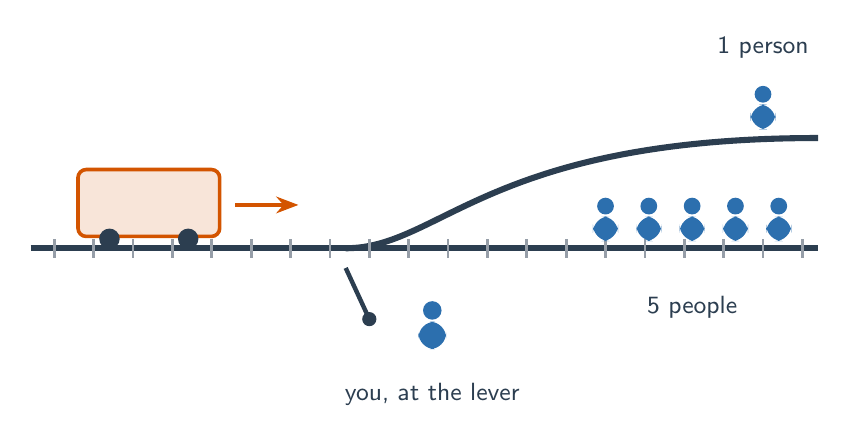
\begin{tikzpicture}[
  lbl/.style={font=\small, text=ink, align=center},
]
% The trolley problem: pull the lever or do nothing.
\draw[ink, line width=2.2pt] (0,0) -- (4,0);
\draw[ink, line width=2.2pt] (4,0) -- (10,0);
\draw[ink, line width=2.2pt] (4,0) .. controls (5.2,0) and (5.8,1.4) .. (10,1.4);
\foreach \x in {0.3,0.8,...,9.8} \draw[ink!50, line width=1pt] (\x,-0.12) -- (\x,0.12);
% trolley (orange: the machine)
\draw[machine, fill=machine!15, line width=1.3pt, rounded corners=3pt] (0.6,0.15) rectangle (2.4,1.0);
\fill[ink] (1.0,0.12) circle (0.13); \fill[ink] (2.0,0.12) circle (0.13);
\draw[flow, draw=machine] (2.6,0.55) -- (3.4,0.55);
% people (blue)
\foreach \x in {7.3,7.85,8.4,8.95,9.5} \personicon{\x}{0.3}{0.38};
\personicon{9.3}{1.72}{0.38}
\node[lbl] at (8.4,-0.75) {5 people};
\node[lbl] at (9.3,2.55) {1 person};
% lever and the person who decides
\draw[ink, line width=1.6pt] (4.3,-0.9) -- (4.0,-0.25);
\fill[ink] (4.3,-0.9) circle (0.09);
\personicon{5.1}{-1.05}{0.42}
\node[lbl] at (5.1,-1.85) {you, at the lever};
\end{tikzpicture}
\end{document}
